
%% sasmoota2017.tex
%% V0.1
%% 26.01.2017
%% by Eveliina Pakarinen
%%
%% This is a skeleton file demonstrating the use of IEEEtran.cls
%% (requires IEEEtran.cls version 1.8b or later) with an IEEE
%% conference paper.


%%*************************************************************************
%% Legal Notice:
%% This code is offered as-is without any warranty either expressed or
%% implied; without even the implied warranty of MERCHANTABILITY or
%% FITNESS FOR A PARTICULAR PURPOSE! 
%% User assumes all risk.
%% In no event shall the IEEE or any contributor to this code be liable for
%% any damages or losses, including, but not limited to, incidental,
%% consequential, or any other damages, resulting from the use or misuse
%% of any information contained here.
%%
%% All comments are the opinions of their respective authors and are not
%% necessarily endorsed by the IEEE.
%%
%% This work is distributed under the LaTeX Project Public License (LPPL)
%% ( http://www.latex-project.org/ ) version 1.3, and may be freely used,
%% distributed and modified. A copy of the LPPL, version 1.3, is included
%% in the base LaTeX documentation of all distributions of LaTeX released
%% 2003/12/01 or later.
%% Retain all contribution notices and credits.
%% ** Modified files should be clearly indicated as such, including  **
%% ** renaming them and changing author support contact information. **
%%*************************************************************************


% *** Authors should verify (and, if needed, correct) their LaTeX system  ***
% *** with the testflow diagnostic prior to trusting their LaTeX platform ***
% *** with production work. The IEEE's font choices and paper sizes can   ***
% *** trigger bugs that do not appear when using other class files.       ***                          ***
% The testflow support page is at:
% http://www.michaelshell.org/tex/testflow/



\documentclass[conference]{sasmoota2017}
% Some Computer Society conferences also require the compsoc mode option,
% but others use the standard conference format.


% Some very useful LaTeX packages include:
% (uncomment the ones you want to load)


% *** MISC UTILITY PACKAGES ***
%
%\usepackage{ifpdf}
% Heiko Oberdiek's ifpdf.sty is very useful if you need conditional
% compilation based on whether the output is pdf or dvi.
% usage:
% \ifpdf
%   % pdf code
% \else
%   % dvi code
% \fi
% The latest version of ifpdf.sty can be obtained from:
% http://www.ctan.org/pkg/ifpdf
% Also, note that IEEEtran.cls V1.7 and later provides a builtin
% \ifCLASSINFOpdf conditional that works the same way.
% When switching from latex to pdflatex and vice-versa, the compiler may
% have to be run twice to clear warning/error messages.






% *** CITATION PACKAGES ***
%
%\usepackage{cite}
% cite.sty was written by Donald Arseneau
% V1.6 and later of IEEEtran pre-defines the format of the cite.sty package
% \cite{} output to follow that of the IEEE. Loading the cite package will
% result in citation numbers being automatically sorted and properly
% "compressed/ranged". e.g., [1], [9], [2], [7], [5], [6] without using
% cite.sty will become [1], [2], [5]--[7], [9] using cite.sty. cite.sty's
% \cite will automatically add leading space, if needed. Use cite.sty's
% noadjust option (cite.sty V3.8 and later) if you want to turn this off
% such as if a citation ever needs to be enclosed in parenthesis.
% cite.sty is already installed on most LaTeX systems. Be sure and use
% version 5.0 (2009-03-20) and later if using hyperref.sty.
% The latest version can be obtained at:
% http://www.ctan.org/pkg/cite
% The documentation is contained in the cite.sty file itself.






% *** GRAPHICS RELATED PACKAGES ***
%
\ifCLASSINFOpdf
  % \usepackage[pdftex]{graphicx}
  % declare the path(s) where your graphic files are
  % \graphicspath{{../pdf/}{../jpeg/}}
  % and their extensions so you won't have to specify these with
  % every instance of \includegraphics
  % \DeclareGraphicsExtensions{.pdf,.jpeg,.png}
\else
  % or other class option (dvipsone, dvipdf, if not using dvips). graphicx
  % will default to the driver specified in the system graphics.cfg if no
  % driver is specified.
  % \usepackage[dvips]{graphicx}
  % declare the path(s) where your graphic files are
  % \graphicspath{{../eps/}}
  % and their extensions so you won't have to specify these with
  % every instance of \includegraphics
  % \DeclareGraphicsExtensions{.eps}
\fi
% graphicx was written by David Carlisle and Sebastian Rahtz. It is
% required if you want graphics, photos, etc. graphicx.sty is already
% installed on most LaTeX systems. The latest version and documentation
% can be obtained at: 
% http://www.ctan.org/pkg/graphicx
% Another good source of documentation is "Using Imported Graphics in
% LaTeX2e" by Keith Reckdahl which can be found at:
% http://www.ctan.org/pkg/epslatex
%
% latex, and pdflatex in dvi mode, support graphics in encapsulated
% postscript (.eps) format. pdflatex in pdf mode supports graphics
% in .pdf, .jpeg, .png and .mps (metapost) formats. Users should ensure
% that all non-photo figures use a vector format (.eps, .pdf, .mps) and
% not a bitmapped formats (.jpeg, .png). The IEEE frowns on bitmapped formats
% which can result in "jaggedy"/blurry rendering of lines and letters as
% well as large increases in file sizes.
%
% You can find documentation about the pdfTeX application at:
% http://www.tug.org/applications/pdftex





% *** MATH PACKAGES ***
%
%\usepackage{amsmath}
% A popular package from the American Mathematical Society that provides
% many useful and powerful commands for dealing with mathematics.
%
% Note that the amsmath package sets \interdisplaylinepenalty to 10000
% thus preventing page breaks from occurring within multiline equations. Use:
%\interdisplaylinepenalty=2500
% after loading amsmath to restore such page breaks as IEEEtran.cls normally
% does. amsmath.sty is already installed on most LaTeX systems. The latest
% version and documentation can be obtained at:
% http://www.ctan.org/pkg/amsmath





% *** SPECIALIZED LIST PACKAGES ***
%
%\usepackage{algorithmic}
% algorithmic.sty was written by Peter Williams and Rogerio Brito.
% This package provides an algorithmic environment fo describing algorithms.
% You can use the algorithmic environment in-text or within a figure
% environment to provide for a floating algorithm. Do NOT use the algorithm
% floating environment provided by algorithm.sty (by the same authors) or
% algorithm2e.sty (by Christophe Fiorio) as the IEEE does not use dedicated
% algorithm float types and packages that provide these will not provide
% correct IEEE style captions. The latest version and documentation of
% algorithmic.sty can be obtained at:
% http://www.ctan.org/pkg/algorithms
% Also of interest may be the (relatively newer and more customizable)
% algorithmicx.sty package by Szasz Janos:
% http://www.ctan.org/pkg/algorithmicx




% *** ALIGNMENT PACKAGES ***
%
%\usepackage{array}
% Frank Mittelbach's and David Carlisle's array.sty patches and improves
% the standard LaTeX2e array and tabular environments to provide better
% appearance and additional user controls. As the default LaTeX2e table
% generation code is lacking to the point of almost being broken with
% respect to the quality of the end results, all users are strongly
% advised to use an enhanced (at the very least that provided by array.sty)
% set of table tools. array.sty is already installed on most systems. The
% latest version and documentation can be obtained at:
% http://www.ctan.org/pkg/array


% IEEEtran contains the IEEEeqnarray family of commands that can be used to
% generate multiline equations as well as matrices, tables, etc., of high
% quality.




% *** SUBFIGURE PACKAGES ***
%\ifCLASSOPTIONcompsoc
%  \usepackage[caption=false,font=normalsize,labelfont=sf,textfont=sf]{subfig}
%\else
%  \usepackage[caption=false,font=footnotesize]{subfig}
%\fi
% subfig.sty, written by Steven Douglas Cochran, is the modern replacement
% for subfigure.sty, the latter of which is no longer maintained and is
% incompatible with some LaTeX packages including fixltx2e. However,
% subfig.sty requires and automatically loads Axel Sommerfeldt's caption.sty
% which will override IEEEtran.cls' handling of captions and this will result
% in non-IEEE style figure/table captions. To prevent this problem, be sure
% and invoke subfig.sty's "caption=false" package option (available since
% subfig.sty version 1.3, 2005/06/28) as this is will preserve IEEEtran.cls
% handling of captions.
% Note that the Computer Society format requires a larger sans serif font
% than the serif footnote size font used in traditional IEEE formatting
% and thus the need to invoke different subfig.sty package options depending
% on whether compsoc mode has been enabled.
%
% The latest version and documentation of subfig.sty can be obtained at:
% http://www.ctan.org/pkg/subfig




% *** FLOAT PACKAGES ***
%
%\usepackage{fixltx2e}
% fixltx2e, the successor to the earlier fix2col.sty, was written by
% Frank Mittelbach and David Carlisle. This package corrects a few problems
% in the LaTeX2e kernel, the most notable of which is that in current
% LaTeX2e releases, the ordering of single and double column floats is not
% guaranteed to be preserved. Thus, an unpatched LaTeX2e can allow a
% single column figure to be placed prior to an earlier double column
% figure.
% Be aware that LaTeX2e kernels dated 2015 and later have fixltx2e.sty's
% corrections already built into the system in which case a warning will
% be issued if an attempt is made to load fixltx2e.sty as it is no longer
% needed.
% The latest version and documentation can be found at:
% http://www.ctan.org/pkg/fixltx2e


%\usepackage{stfloats}
% stfloats.sty was written by Sigitas Tolusis. This package gives LaTeX2e
% the ability to do double column floats at the bottom of the page as well
% as the top. (e.g., "\begin{figure*}[!b]" is not normally possible in
% LaTeX2e). It also provides a command:
%\fnbelowfloat
% to enable the placement of footnotes below bottom floats (the standard
% LaTeX2e kernel puts them above bottom floats). This is an invasive package
% which rewrites many portions of the LaTeX2e float routines. It may not work
% with other packages that modify the LaTeX2e float routines. The latest
% version and documentation can be obtained at:
% http://www.ctan.org/pkg/stfloats
% Do not use the stfloats baselinefloat ability as the IEEE does not allow
% \baselineskip to stretch. Authors submitting work to the IEEE should note
% that the IEEE rarely uses double column equations and that authors should try
% to avoid such use. Do not be tempted to use the cuted.sty or midfloat.sty
% packages (also by Sigitas Tolusis) as the IEEE does not format its papers in
% such ways.
% Do not attempt to use stfloats with fixltx2e as they are incompatible.
% Instead, use Morten Hogholm'a dblfloatfix which combines the features
% of both fixltx2e and stfloats:
%
% \usepackage{dblfloatfix}
% The latest version can be found at:
% http://www.ctan.org/pkg/dblfloatfix




% *** PDF, URL AND HYPERLINK PACKAGES ***
%
%\usepackage{url}
% url.sty was written by Donald Arseneau. It provides better support for
% handling and breaking URLs. url.sty is already installed on most LaTeX
% systems. The latest version and documentation can be obtained at:
% http://www.ctan.org/pkg/url
% Basically, \url{my_url_here}.




% *** Do not adjust lengths that control margins, column widths, etc. ***
% *** Do not use packages that alter fonts (such as pslatex).         ***
% There should be no need to do such things with IEEEtran.cls V1.6 and later.
% (Unless specifically asked to do so by the journal or conference you plan
% to submit to, of course. )

\usepackage{graphicx}
\usepackage[export]{adjustbox}

% correct bad hyphenation here
\hyphenation{op-tical net-works semi-conduc-tor}


\begin{document}
%
% paper title
% Titles are generally capitalized except for words such as a, an, and, as,
% at, but, by, for, in, nor, of, on, or, the, to and up, which are usually
% not capitalized unless they are the first or last word of the title.
% Linebreaks \\ can be used within to get better formatting as desired.
% Do not put math or special symbols in the title.
\title{Multi-tenancy in Software as a Service Applications}


% author names and affiliations
% use a multiple column layout for up to three different
% affiliations
\author{\IEEEauthorblockN{Eveliina Pakarinen}
\IEEEauthorblockA{University of Helsinki\\
Helsinki, Finland}}


% make the title area
\maketitle

% As a general rule, do not put math, special symbols or citations
% in the abstract
\begin{abstract}
Multi-tenancy is a high level architectural pattern which can be used in cloud computing environment when offering applications using Software as a Service business model. In multi-tenancy pattern service provider hosts a single instance of an application on his or her infrastructure and this application is accessed by multiple tenants who share the resources of the infrastructure. The use of multi-tenancy pattern brings multiple benefits both to the service provider and to the customers but there are also some complexities that affect the use of multi-tenancy. Although multi-tenancy is a popular paradigm it is still a relatively new topic in scientific literature and the research domain of multi-tenancy is not yet mature which can be seen from the lack of industrial experience reports on multi-tenancy. In this paper the key concepts of multi-tenancy in SaaS applications are presented and some concerns that need to be taken into account when developing a multi-tenant SaaS application are discussed. A couple of recently proposed example frameworks for developing multi-tenant applications are also presented in order to describe the current situation in multi-tenancy research.

\end{abstract}

% no keywords

Keywords: multi-tenancy, Software as a Service, architectural pattern



\IEEEpeerreviewmaketitle



\section{Introduction}
\textit{Software as a Service} (SaaS) is a software delivery and business model where an application is provided as an on-demand service for multiple users through Internet \cite{Kang:2011:DesignOfConceptual}. In SaaS business model the service provider maintains the application and offers the software as a service to the customers \cite{Bezemer:2010:MaintenanceDream}. By using software offered by a third party companies can use various IT services without maintaining or purchasing their own IT infrastructure \cite{Bezemer:2010:MaintenanceDream}. 

\textit{Multi-tenancy} is a high level architectural pattern which can be used when offering applications as Software as a Service in cloud computing environment \cite{Kabbedijk2015:Defining}. In multi-tenancy pattern the service provider hosts a single instance of the software product on his or her infrastructure and multiple customers, so called tenants, access the same instance of the software \cite{Bezemer:2010:MaintenanceDream}. A tenant is the organizational entity which rents a multi-tenant SaaS solution \cite{Bezemer:2010:MaintenanceDream}. A tenant groups typically multiple users of the same organization and these users are the stakeholders in the organization. 

There are multiple benefits for the service provider when using multi-tenant architecture pattern when implementing SaaS applications. The first benefit is that the application deployment becomes easier because only one application instance has to be deployed \cite{Bezemer:2010:MaintenanceDream}. In multi-tenant model multiple customers access the same software instance and they do not need own dedicated instance of the software. This means that the customers share the same hardware resources when using multi-tenant SaaS application \cite{Pal:2015:ApplicationMultiTenancy}. That increases and improves the utilization rate of the hardware which is the second benefit of the multi-tenant model \cite{Bezemer:2010:MaintenanceDream}. 

These two benefits reduce the software delivery costs for the service provider which can help improve the profit margin \cite{Guo:2007:FrameworkForNative}. The reduced delivery costs enable that software provider can offer the service to the customers at lower service subscription costs \cite{Guo:2007:FrameworkForNative}. That makes multi-tenant applications interesting for customers in the small and medium enterprise segment \cite{Bezemer:2010:MaintenanceDream}.

In addition to the benefits of the multi-tenancy there are also some complexities that come with the multi-tenancy. Challenges can arise in the application development, deployment and management phases \cite{Guo:2007:FrameworkForNative}. Challenges that arise are for example application performance, scalability, security, zero-downtime and maintenance \cite{Bezemer:2010:MaintenanceDream}.

Although multi-tenancy is a popular paradigm it is still a relatively new topic in scientific literature \cite{Kabbedijk2015:Defining}. The term ‘multi-tenancy’ was explicitly mentioned for the first time in a scientific paper in year 2006. Since then many definitions for multi-tenancy have been proposed \cite{Kabbedijk2015:Defining}. Also many solutions related to multi-tenancy have been proposed in the multi-tenancy research over the years but there has been very few industrial reports about experiences on multi-tenancy \cite{Kabbedijk2015:Defining}. This indicates that the research domain of multi-tenancy is not yet mature and that the solutions have not yet been implemented or evaluated. The high amount of proposals and the low amount of industrial reports can also indicate that there is a lack of cooperation between industry and academia in this domain \cite{Kabbedijk2015:Defining}.

In this paper the key concepts of multi-tenancy in SaaS applications are presented and some concerns that need to be taken into account when developing a multi-tenant SaaS application are discussed. A couple of recently proposed example frameworks for developing a multi-tenant applications are also presented in order to describe the current situation in multi-tenancy research.
 
This paper is organized as follows. In Section 2 the research methods for data collection for this paper are introduced and the research questions are presented. In section 3 an introduction to multi-tenancy and SaaS is given. In section 4 an example architecture framework for multi-tenant architecture is presented. In section 5 the answers to the research questions are discussed. A conclusion is presented in section 6. 


%\cite{Kabbedijk2015:Defining}
%\cite{Bezemer:2010:MaintenanceDream}
%\cite{Weissman:2009:Forcecom}
%\cite{Guo:2007:FrameworkForNative}
%\cite{Kang:2011:DesignOfConceptual}
%\cite{Pal:2015:ApplicationMultiTenancy}
%\cite{Schroeter:2012:TowardsModeling}
%\cite{Samrajesh:2016:ScalableComponent}
%\cite{Bien:2015:MultiTenantWebApp}
%\cite{Bezemer:2010:EnablingMultiTenancy}
%\cite{Ru:2014:SoftareEngineering}
%\cite{Vidhyalakshmi:2014:DesignComparison}
%\cite{Mietzner:2009:VariabilityModeling}


%\hfill mds
% 
%\hfill January 26, 2017
%
%\subsection{Clever Subsection Header}
%My own subsection
%
%
%\subsubsection{Clever Subsection Header}
%My clever subsection text


% An example of a floating figure using the graphicx package.
% Note that \label must occur AFTER (or within) \caption.
% For figures, \caption should occur after the \includegraphics.
% Note that IEEEtran v1.7 and later has special internal code that
% is designed to preserve the operation of \label within \caption
% even when the captionsoff option is in effect. However, because
% of issues like this, it may be the safest practice to put all your
% \label just after \caption rather than within \caption{}.
%
% Reminder: the "draftcls" or "draftclsnofoot", not "draft", class
% option should be used if it is desired that the figures are to be
% displayed while in draft mode.
%
%\begin{figure}[!t]
%\centering
%\includegraphics[width=2.5in]{myfigure}
% where an .eps filename suffix will be assumed under latex, 
% and a .pdf suffix will be assumed for pdflatex; or what has been declared
% via \DeclareGraphicsExtensions.
%\caption{Simulation results for the network.}
%\label{fig_sim}
%\end{figure}

% Note that the IEEE typically puts floats only at the top, even when this
% results in a large percentage of a column being occupied by floats.


% An example of a double column floating figure using two subfigures.
% (The subfig.sty package must be loaded for this to work.)
% The subfigure \label commands are set within each subfloat command,
% and the \label for the overall figure must come after \caption.
% \hfil is used as a separator to get equal spacing.
% Watch out that the combined width of all the subfigures on a 
% line do not exceed the text width or a line break will occur.
%
%\begin{figure*}[!t]
%\centering
%\subfloat[Case I]{\includegraphics[width=2.5in]{box}%
%\label{fig_first_case}}
%\hfil
%\subfloat[Case II]{\includegraphics[width=2.5in]{box}%
%\label{fig_second_case}}
%\caption{Simulation results for the network.}
%\label{fig_sim}
%\end{figure*}
%
% Note that often IEEE papers with subfigures do not employ subfigure
% captions (using the optional argument to \subfloat[]), but instead will
% reference/describe all of them (a), (b), etc., within the main caption.
% Be aware that for subfig.sty to generate the (a), (b), etc., subfigure
% labels, the optional argument to \subfloat must be present. If a
% subcaption is not desired, just leave its contents blank,
% e.g., \subfloat[].


% An example of a floating table. Note that, for IEEE style tables, the
% \caption command should come BEFORE the table and, given that table
% captions serve much like titles, are usually capitalized except for words
% such as a, an, and, as, at, but, by, for, in, nor, of, on, or, the, to
% and up, which are usually not capitalized unless they are the first or
% last word of the caption. Table text will default to \footnotesize as
% the IEEE normally uses this smaller font for tables.
% The \label must come after \caption as always.
%
%\begin{table}[!t]
%% increase table row spacing, adjust to taste
%\renewcommand{\arraystretch}{1.3}
% if using array.sty, it might be a good idea to tweak the value of
% \extrarowheight as needed to properly center the text within the cells
%\caption{An Example of a Table}
%\label{table_example}
%\centering
%% Some packages, such as MDW tools, offer better commands for making tables
%% than the plain LaTeX2e tabular which is used here.
%\begin{tabular}{|c||c|}
%\hline
%One & Two\\
%\hline
%Three & Four\\
%\hline
%\end{tabular}
%\end{table}


% Note that the IEEE does not put floats in the very first column
% - or typically anywhere on the first page for that matter. Also,
% in-text middle ("here") positioning is typically not used, but it
% is allowed and encouraged for Computer Society conferences (but
% not Computer Society journals). Most IEEE journals/conferences use
% top floats exclusively. 
% Note that, LaTeX2e, unlike IEEE journals/conferences, places
% footnotes above bottom floats. This can be corrected via the
% \fnbelowfloat command of the stfloats package.



\section{Research methods}

This seminar work is based on academic papers published in various conferences and journals. The search for these papers was mainly done in the ACM Digital Library and in the IEEE Xplore Digital Library. Initial search criteria for papers were that the paper was published recently between years from 2014 to 2016 and that the paper had something to do with multi-tenancy and architecture or multi-tenancy and SaaS applications or generally mentioned multi-tenancy. After finding a couple of papers the references in them were used to find more papers related to the theme discussed in the paper. Web of Science was also used to find papers that had cited the papers found during the search in digital libraries. 

The initial goal for data collection was to find as many papers as possible. After that the first thing to do was to filter out papers that were not suitable as sources for this seminar work. Characteristics for not suitable papers were for example that the paper was published in a too small conference or unknown journal or that it did not discuss multi-tenancy in application level in SaaS applications or that multi-tenancy was not discussed from architectural perspective. 

After that the remaining papers were organized to four groups based on the abstract, introduction and conclusion parts of the papers. The groups in which the papers were organized were: 

\begin{enumerate}
\item not so relevant papers for this seminar work
\item important papers for this seminar work
\item papers that propose some multi-tenant pattern or architecture 
\item supporting papers with relevant background information.
\end{enumerate}
The papers that belonged to group 1 were left out and the papers that belonged to groups 2, 3 and 4 were studied further. The references that are used in this seminar work are based on the papers that belonged to groups 2, 3 and 4.

The main research questions for this seminar work are: What is multi-tenancy and what does it have to do with SaaS applications? What kind of architecture frameworks have been proposed for multi-tenant applications? What needs to be taken into consideration when developing multi-tenant applications? This seminar paper also tries to provide a clear description of multi-tenancy and multi-tenant SaaS applications.

\section{Introduction to multi-tenancy and SaaS (software/architecture/patterns)}

Multi-tenancy is a high level architectural pattern which can be used to share computing resources when offering software products as Software as a Service \cite{Kabbedijk2015:Defining}. In multi-tenancy a single instance of an application is hosted on service provider’s infrastructure and this single instance is accessed by multiple tenants and can be customized according to the requirements of different tenants \cite{Kabbedijk2015:Defining}. Multi-tenancy has evolved from previous information technology paradigms like time-sharing, application service provider (ASP) model and multi-user model \cite{Kabbedijk2015:Defining}. Multi-tenancy was explicitly mentioned in scientific literature for the first time in the domain of software and hardware systems in year 2006 \cite{Kabbedijk2015:Defining}. 

In academic literature the definition of multi-tenancy has been varying and there has been differences in the interpretation of multi-tenancy among academics in academia \cite{Kabbedijk2015:Defining}. In order to chart and bridge the varying definitions of multi-tenancy and to provide an overview of the multi-tenancy domain Kabbedijk et al. \cite{Kabbedijk2015:Defining} performed a structural search in academic literature and blog posts. They propose a comprehensive definition for multi-tenancy which is based on the definitions of multi-tenancy presented in academic literature \cite{Kabbedijk2015:Defining}. Their definition of multi-tenancy is: “Multi-tenancy is a property of a system where multiple customers, so-called tenants, transparently share the system’s resources, such as services, applications, databases, or hardware, with the aim of lowering costs, while still being able to exclusively configure the system to the needs of the tenant \cite{Kabbedijk2015:Defining}.”

In Figure 1 different system levels are illustrated in different variants of multi-tenancy and in single-tenancy for two tenants. In Figure 1 the system levels marked with yellow background color represent application and software levels of the system. The infrastructure levels of the system are marked with purple background color and the database levels are marked with green background color. The levels of the system that are influenced by software level multi-tenancy are marked with solid borders and bold font style. Those levels are application instance, application server, database schema, database and database server \cite{Kabbedijk2015:Defining}. The levels that are not influenced by software level multi-tenancy are middleware, operating system, virtual machine and hardware and those levels are marked with dashed line borders and plain font style in Figure 1. 

In native or pure multi-tenancy \cite{Kabbedijk2015:Defining, Guo:2007:FrameworkForNative} the tenants share the same application instance and database tables which are hosted on a shared infrastructure. Native multi-tenancy variant is used to support a large number of tenants and the number is usually in the hundreds or thousands of tenants \cite{Guo:2007:FrameworkForNative}. 

In the semi-multi-tenancy variants of multi-tenancy the tenants share the same application instance but the level of sharing on the database levels of the system vary. The two variants of semi-multi-tenancy are “shared application, shared database and separate table” -variant and “shared application and separate database” -variant \cite{Bezemer:2010:MaintenanceDream}. When a high number of tenants are placed on the same server and one of the semi-multi-tenancy variants of multi-tenancy is used it can cause performance problems on the server \cite{Bezemer:2010:MaintenanceDream}. These performance problems are caused by the expensive operation of loading a database or table in memory when a tenant accesses the application. When comparing this to native multi-tenancy native multi-tenancy enables placing more tenants on the same the server because the shared database table must be loaded only once to memory \cite{Bezemer:2010:MaintenanceDream}.

In multiple instances multi-tenancy tenants no longer share the same application instance. Instead of sharing an application instance each tenant has its own dedicated application instance over a shared middleware server, operating system or hardware \cite{Guo:2007:FrameworkForNative}. Two variants of multiple instances multi-tenancy are presented in the Figure 1. Multiple instances multi-tenancy variants scale differently than native multi-tenancy when comparing the number of tenants which multiple instances variants or native multi-tenancy can support \cite{Guo:2007:FrameworkForNative}. Multiple instances multi-tenancy variants can support several up to dozens of tenants while native multi-tenancy can support hundreds or thousands of tenants \cite{Guo:2007:FrameworkForNative}.

\begin{figure}
	\centering
		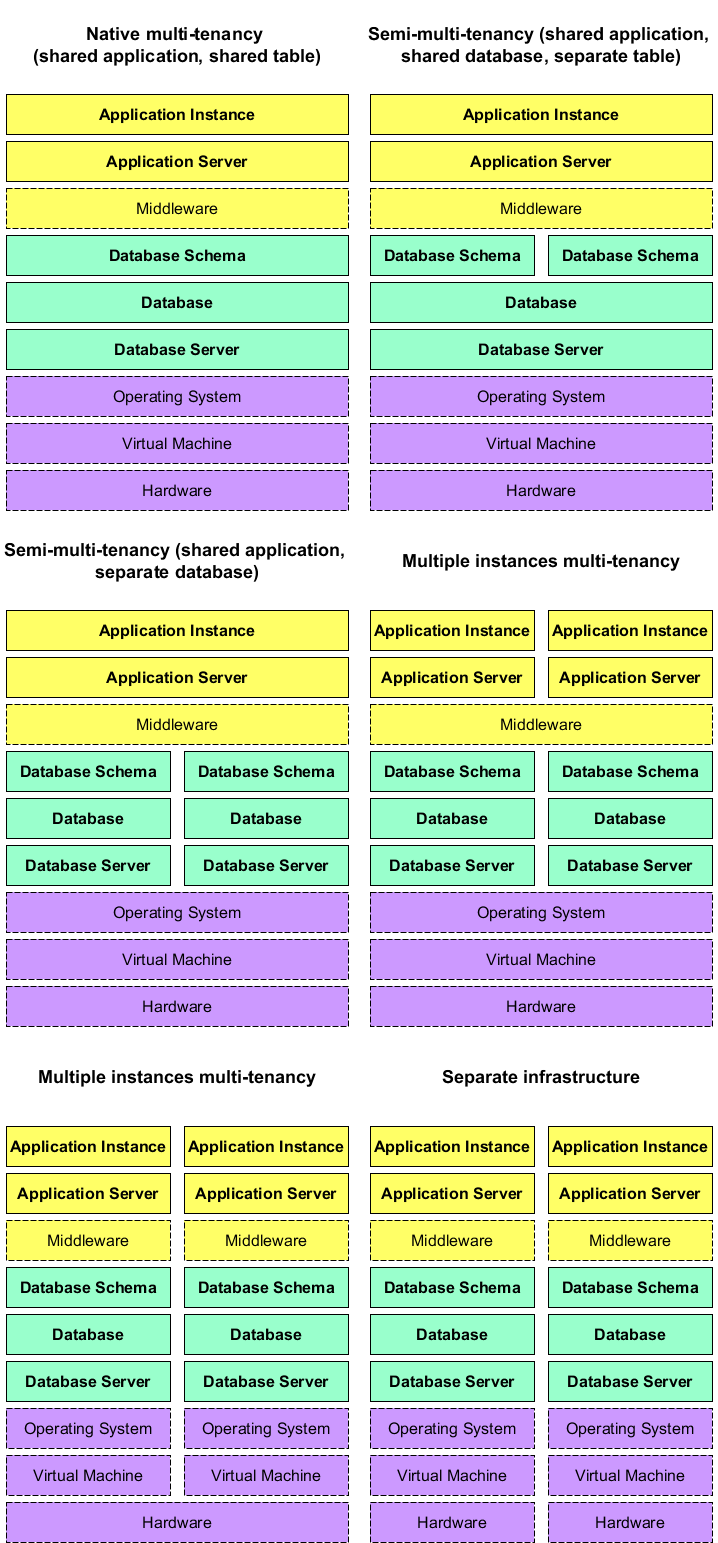
\includegraphics[max size={0.8\textwidth}{0.8\textheight}]{MTvsMILong}
	\caption{Illustration of different system levels in different variants of multi-tenancy and in single-tenancy.}
	\label{figure:MTvsMILong}
\end{figure}

As a comparison point to different multi-tenancy variants a single-tenancy approach is also presented in Figure 1. In traditional single-tenant approach each tenant has own dedicated server and own customized application instance which they use \cite{Bezemer:2010:MaintenanceDream}. This means that single-tenant application may have many separate running instances which all can be different from each other \cite{Bezemer:2010:MaintenanceDream}. A traditional single-tenancy scenario from the early 90s was that companies moved their hardware and applications from their premises to data centers where the applications were hosted without any hardware or software sharing \cite{Guo:2007:FrameworkForNative}. 

In single-tenancy server utilization can be low especially when applications are used by customers in the small and medium enterprise (SME) segment of the market \cite{Bezemer:2010:MaintenanceDream}. In that situation server utilization can be improved by placing several tenants on the same server \cite{Bezemer:2010:MaintenanceDream}. Different multi-tenancy variants from multiple instances multi-tenancy to native multi-tenancy can be used to place several tenants on the same server which improves the utilization of the servers. Through higher utilization of the servers the total amount of hardware required to serve the tenants is lower than when using single-tenancy where each tenant has its own dedicated server. The result of requiring lower amount of hardware because of higher server utilization in multi-tenancy is that the overall costs of the application will be lower \cite{Bezemer:2010:MaintenanceDream}.


\section{Results: Evaluation/validation/review of a proposed architecture pattern/framework for multi-tenant SaaS application}
(or maybe comparison to some other framework? How has it evolved through years?) 

Answers to the research questions (should be here?)

New results

Neutral analysis based on the data. New ideas/new things/ 
new viewpoints based on the material → my unique way to combine the materials to something new? 

\section{Discussion}
How well the research questions were answered?

Discuss my answers to research questions

Limitations that affect the validity of the results

Related work or comparison to other work (maybe)

\section{Conclusion}
Main points, message

Probably some mention about future work or what should be researched next






% trigger a \newpage just before the given reference
% number - used to balance the columns on the last page
% adjust value as needed - may need to be readjusted if
% the document is modified later
%\IEEEtriggeratref{8}
% The "triggered" command can be changed if desired:
%\IEEEtriggercmd{\enlargethispage{-5in}}

% references section

% can use a bibliography generated by BibTeX as a .bbl file
% BibTeX documentation can be easily obtained at:
% http://mirror.ctan.org/biblio/bibtex/contrib/doc/
% The IEEEtran BibTeX style support page is at:
% http://www.michaelshell.org/tex/ieeetran/bibtex/
%\bibliographystyle{IEEEtran}
% argument is your BibTeX string definitions and bibliography database(s)
%\bibliography{IEEEabrv,../bib/paper}
%
% <OR> manually copy in the resultant .bbl file
% set second argument of \begin to the number of references
% (used to reserve space for the reference number labels box)



%\begin{thebibliography}{1}
%
%\bibitem{IEEEhowto:kopka}
%H.~Kopka and P.~W. Daly, \emph{A Guide to \LaTeX}, 3rd~ed.\hskip 1em plus
%  0.5em minus 0.4em\relax Harlow, England: Addison-Wesley, 1999.
%

\bibliographystyle{IEEEtran}
\bibliography{IEEEabrv,sasmoota2017}
%\end{thebibliography}




\end{document}


